\chapter{Pipeline extraction} \label{chapter5}

The previous chapter presented globally the state of the art in designing systems to scale in performance, and in maintenance.
It refined the scope of this thesis to the study of the opposition between maintenance scalability and performance scalability in streaming web applications.
It concluded with the objectives of this thesis, which is to find an equivalence between the two opposed organizations.
The maintenance scalability organization, supported by modular programming, higher-order programming and a global memory store.
The performance scalability organization, supported by the parallelism of memory and exuction distribution.
The equivalence between these two organization is in two steps, as presented in figure \ref{fig:chapter3:objectives:roadmap}.
This chapter presents the first step in this equivalence.
That is to identify and extract a pipeline of execution inside an application following the first organization.
In this work, we focus on Javascript, and specifically node.js applications.
In this chapter, I define further the higher-order programming concepts.

In Javascript, functions are first-class citizens ; it allows to manipulate them like any object, and to link them to react to asynchronous events, \textit{e.g.} user inputs and remote requests.
These asynchronously triggered functions are named callbacks, and allow to efficiently cope with the distributed and inherently asynchronous architecture of the Internet.
To execute a suite of asynchronous functions, callbacks are nested one into the other.
This nesting, if not organized properly, can result in unreadable layer of callbacks, commonly presented as \textit{callback hell}\ftnt{http://maxogden.github.io/callback-hell/}, or \textit{pyramid of doom}.

Promises are another way to organize a suite of asynchronous operations avoiding this callback hell.
They organize the operations as a well-defined pipeline.
Moreover, Promises provide additional control over the asynchronous execution flow, than callbacks.
They are part of the next version of the Javascript language, ECMAScript 6\ftnt{http://people.mozilla.org/~jorendorff/es6-draft.html}.
To avoid the equivalence being unnecessarily incomplete, we present an alternative to Promise, called Due.
Due organize the operations like Promises, as a well-defined pipeline, while discarding the unnecessary additional control over the asynchronous flow.

This chapter present an equivalence, and a compiler to identify the pipeline of operating underlying in a Javascript application using callbacks, and extract it to express it as Dues.
This compiler has been tested over 64 \textit{Node.js} packages from the node package manager (npm\ftnt{https://www.npmjs.com/}).
55 packages were incompatible with the compiler, 9 packages were compiled with success.

Callbacks, Promises and Dues are further defined in section \ref{section:definitions}.
Section \ref{section:equivalence} explains the transformation from imbrications of callbacks to sequences of Dues.
Section \ref{section:compiler} presents a compiler to automate the application of this equivalence.
And finally, the developed compiler is evaluated in section \ref{section:evaluation}.


% This made Javascript a language of choice to develop both client and, more recently, server applications for the web.

% Callbacks are well-suited for small interactive scripts.
% But in a complete application, they are ill-suited to control the larger asynchronous execution flow.
% Their use leads to intricate imbrications of function calls and callbacks, commonly presented as \textit{callback hell}\ftnt{http://maxogden.github.io/callback-hell/}, or \textit{pyramid of doom}.
% This is widely recognized as a bad practice and reflects the unsuitability of callbacks in complete applications.
% Eventually, developers enhanced callbacks to meet their needs with the concept of Promise~\cite{Liskov1988}.

% Promises bring a different way to control the asynchronous execution flow, better suited for large applications.
% They fulfill this task well enough to be part of the next version of the Javascript language, ECMAScript 6\ftnt{http://people.mozilla.org/~jorendorff/es6-draft.html}.
% However, because Javascript started as a scripting language, beginners are often not introduced to Promises early enough.
% Most APIs use the classical callback approach encouraging beginner in this practice.
% Moreover, despite its benefits, the concept of Promise is not yet widely acknowledged.
% Developers may implement their own library for asynchronous flow control before discovering existing ones.
% There is such a disparity between the needs for and the adoption of Promises libraries, that there are almost 40 different implementations\ftnt{https://github.com/promises-aplus/promises-spec/blob/master/implementations.md}.

% With the upcoming introduction of Promise as a language feature, we expect an increase of interest, and believe that many developers will shift to this better practice.
% In this paper, we propose a compiler to automate this shift in existing code bases.
% We present the transformation from an imbrication of callbacks to a sequence of Promise operations, while preserving the semantic.

% Promises bring a better way to control the asynchronous execution flow, but they also impose a conditional control over the result of the execution.
% Callbacks, on the other hand, leave this conditional control to the developer.
% This paper focuses on the transformation from imbrication of callbacks to chain of Promises.
% To avoid unnecessary modifications on this conditional control, we introduce an alternative to Promises leaving this conditional control to the developer, like callbacks.
% We call this simpler specification Dues.
% Our approach enables us to compile legacy Javascript code and brings a first automated step toward full Promises integration.
% This simple and pragmatic compiler has been tested over 64 \textit{Node.js} packages from the node package manager (npm\ftnt{https://www.npmjs.com/}), 9 of them with success.

% In section \ref{section:definitions} we define callbacks, Promises and Dues.
% In section \ref{section:equivalence}, we explain the transformation from imbrications of callbacks to sequences of Dues.
% In section \ref{section:compiler}, we present a compiler to automate the application of this equivalence.
% In section \ref{section:evaluation}, we evaluate the developed compiler.

\section{Definitions} \label{chapter3:definitions}

The continuous growth and sustainability offered by a platform relies on three criteria.
This section defines these tree criteria, as well as all the underlying concepts.

Additionally, for the context of this thesis, a fourth criterium appear.
It is important for the analyzed platforms to be web compliant.\nt{I don't know where to put this criterium}

\begin{itemize}
\item Maintainability
\item Performance Efficiency
\item Adoption
\item Web compliance
\end{itemize}

\subsection{Maintainability}

\textit{Software maintainability is defined as the degree to which an application is understood, repaired, or enhanced.}\ftnt{http://www.castsoftware.com/glossary/software-maintainability}
% For an application to be maintainable, it needs to be modular.
%Maintainability relies on modularity.
For an application to be maintainable, its frameworks need to enforce modularity directly in the design.
Modularity allows to limit the understanding required to contribute to a module \cite{Stevens1974}.
Which helps developers to repair and enhance the application. 
Moreover, it reduces development time by allowing several developers to simultaneously implement different modules \cite{Wong2009,Cataldo2006}.
% It relies on two factors, module encapsulation and module composition.

\subsubsection{Modularity}

The modularity of a software implementation is about encapsulating subproblems and composing them.
It allows greater design to emerge from the composition of smaller components.

The criteria to define modules to improve maintainability are low coupling and high cohesion \cite{Stevens1974}.
Coupling defines the strength of the interdependence between modules.
Cohesion defines how strongly the features inside a module are related.
% Encapsulating a subproblem into a module helps increase cohesion.
% Composition abstractions helps decrease their coupling.
The composition of modules help decrease coupling, and encapsulation helps increase their cohesion.
Encapsulation and composition improves maintainability.

\begin{itemize}
\item Encapsulation $\to$ High Cohesion
\item Composition $\to$ Low Coupling
\end{itemize}

\subsubsection{Encapsulation}

\paragraph{Boundary Definition}

\illustration{spaghetti programming}
Modular Programming stands upon Structured Programming \cite{Dijkstra1970}.
% Dijkstra firstly developed the concept of Structured Programming \cite{Dijkstra1970}, which later led to modular programming.
% It is defined as \textit{the systematic use of abstraction to control a mass of details, and also a means of documentation which aids program design} \cite{Knuth1974}.
It draws clear interfaces around a piece of implementation so that the execution is enclosed inside.
At a fine level, it helps avoid spaghetti code \cite{Dijkstra1968a}, and at a coarser level, it structures the implementation \cite{Dijkstra1968} into modules, or layers.
% The next paragraph explains further the criteria to draw the borders around modules.

\paragraph{Data Protection}

\illustration{lasagna programming}
Encapsulate a specific design choice in each module, so that it is responsible for one and only one concern, isolate its evolution from impacting the rest of the implementation \cite{Parnas1972, Tarr1999, Hursch1995}.
Examples of such separation of concerns are the separation of the form and the content in HTML / CSS, or the OSI model for the network stack.

\subsubsection{Composition} \label{chapter3:software-maintainability:modularity:features}

\paragraph{Higher-Order Programming}
\nt{If possible, include this reference : Continuations and coroutines \cite{Haynes1984}}

Higher-order programming allows to manipulate functions like any other primary value : to store them in variables, or to pass them as arguments.
It replaces the need for most modern object oriented programming design patterns \ftnt{http://stackoverflow.com/a/5797892/933670} with Inversion of Control \cite{Johnson}, the Hollywood Principle \cite{Sweet1985}, and Monads \cite{Wadler1992}.
Higher-order programming help loosen coupling, thus improve maintainability.

In languages allowing mutable state, higher-order functions are implemented as closure, to preserve the lexical scope \cite{Sussman1998}.
A closure is the association of a function and a reference to the lexical context from its creation.
It allows this function to access variable from this context, even when invoked outside the scope of this context.
\nt{next sentence is redundant with the suit}
It eventually tangles the memory references so that it requires a global memory.

\paragraph{Lazy Evaluation}

Lazy evaluation is an evaluation strategy allowing to defer the execution of a function only when its result is needed.
% And according to \cite{Hughes1989}, \textit{Abelson and Sussman stress that streams (lazy list) is a powerful tool for structuring programs \cite{Sussman1983}.
The lazy evaluation of lists is equivalent to a stream with a null-sized buffer, while the opposite, eager evaluation, corresponds to an infinite buffer \cite{VanRoy2003}.
\nt{find another transition}Indeed, the dataflow programming paradigm resulting from lazy lists is particularly adapted for stream processing applications.

\nt{This paragraph is not very clear}
The lazy evaluation, as well as streams are powerful tools for structuring modular programs \cite{Sussman1983}.
Lazy evaluation allows the execution to be organized as a concurrent pipeline, as the stages are executed independently for each element of the stream.
But this concurrency requires immutability of state, or at least isolation of side-effects.\nt{why ? explain or point to the explanation}
The next section addresses the consequences of higher-order programming and lazy evaluation on parallelism.



\paragraph{}

Finally, the criteria for Maintainability are the following.

\begin{itemize}
\item Encapsulation $\to$ High Cohesion
  \subitem Boundary definition
  \subitem Data protection
\item Composition $\to$ Low Coupling
  \subitem Higher-order programming, Lambda Expressions
  \subitem Lazy evaluation, Stream composition
\end{itemize}


\subsection{Performance Efficiency}

The performance efficiency of a software project is the relation between the usage made of available resources and the delivered performance.
For an application to perform efficiently, the frameworks used need to enforce scalability directly in its design.

Scalability relies on the commutativity of operations execution \cite{Clements2013a}.
Operations are commutative if the order of their executions is irrelevant for the correctness of their results.
Commutativity assures the independence of operations.

\subsubsection{Independence}

The independence, and commutativity of an operations depends on its access to state shared with other operations.
If the operations doesn't rely on any shared state, it is independent.
If it relies on shared state for read or modification, it needs to manage the timing of its execution with the other operations to avoid conflicting accesses.
That is to synchronize with the other operations, which implies communications.

The independence of operations allows to execute them in parallel, hence to deliver performance proportionally to used resources \cite{Amdahl1967,Gunther1993}.
But if the operations are not independent, the communication overhead due to synchronization might occult the performance increase gained by the parallel execution.
If the two operations frequently access the state, then the communications overhead is greater than the performance gain.
On the other hand, if the operations hardly ever access the state, then the communication overhead is compensated by the performance gain.
Because states tend to be shared locally, the operations at a fine-grain level induce a greater communication overhead than the operations at a coarser-level. 
% \subsubsection{Sequentiality or Parallelism}
% In practice, all operations can not be made independent, particularly at a fine-grain level.
% Enforcing parallelism at this fine-grain level induces overhead because of the synchronization between operations.

Therefore, performance efficiency requires the combination of fine-level state sharing to avoid communication overhead, and coarse-level independence to avoid synchronization overhead \cite{Gustafson1988,Gunther1996,Nelson1996,Gunther2002}.
The operations need to be independent at a coarse-grain level, and to be scheduled sequentially at a fine-grain level.

\begin{itemize}
\item Fine-level state sharing\\
  \subitem State mutability
  \subitem $\to$ Sequentiality
\item Coarse-level independence\\
  \subitem State immutability
  \subitem $\to$ Message-passing
\end{itemize}

\subsubsection{Atomicity, Concurrency and Asynchronism}
TODO

\subsubsection{Message-Passing}
TODO


\subsubsection{Modules and Operations}

On the difference between modules encapsulation and operations independence.

Encapsulation aims not to provide this decomposition between sharing and immutable space required for performance scalability.
It aims to draw a clear boundary around the concern of a module to help understanding it.
To allow higher-order programming and mutable state, despite encapsulation, languages implement closures, and intermingle the memory between modules.
It reinforces the need for synchronization and sequentiality.






\subsection{Adoption}

% A software project is maintainable only if there is people willing to maintain it.
An application is sustainable only if the frameworks used to build it generate activity between a community of passionate and the industry.
A framework needs to present a balance between maintainability and performance effiency to be adopted by both the community and the industry.
The maintainability is required for a framework to be appealing to gather a community to support the ecosystem around it.
And the performance efficiency is required to be economically viable and needed by the industry, and to provide the reason for this ecosystem to exist.

\begin{itemize}
\item Community Support
\item Industrial Need
\end{itemize}

This incitation to balance between maintainability and performance efficiency is illsutrated in figure \ref{fig:state-of-the-art}.

\begin{figure}[h!] \label{fig:state-of-the-art}
\begin{center}
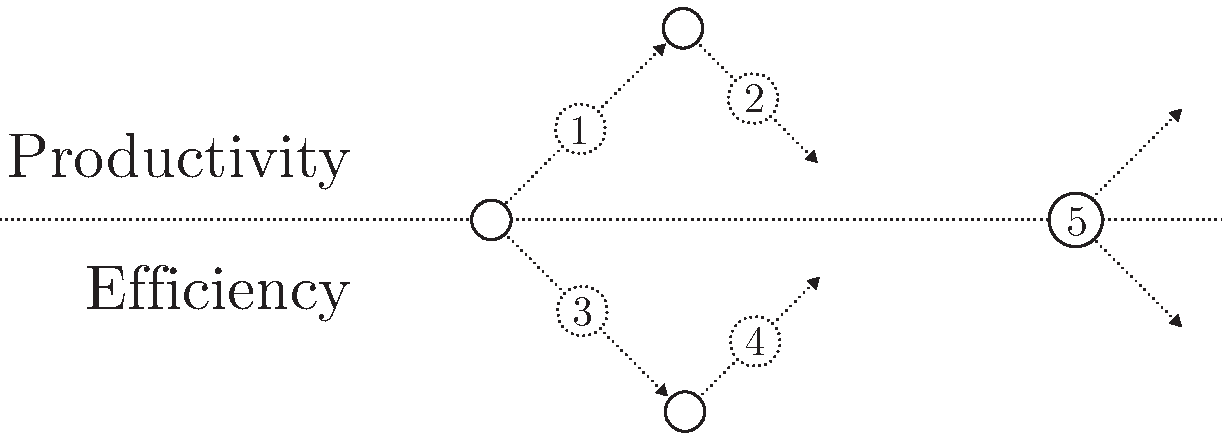
\includegraphics[width=0.6\textwidth]{../ressources/state-of-the-art.pdf}
\end{center}
\end{figure}

\subsection{Web Compliance}

TODO





\section{Equivalence} \label{chapter4:equivalence}

The goal of this thesis is not to propose a new high-level language but to automate the architectural shift.
The next paragraphs introduces the equivalence between the memory abstraction of the event-driven execution model and of the pipeline architecture previously presented.
The equivalence is broken down in two steps, as illustrated in figure \ref{fig:chapter4:roadmap}.
The first step identifies the stages of the pipeline and the rupture points between them in the control flow.
The second step enforces isolation of memory between these stages to preserve invariance.

\begin{figure}[h!]
\begin{center}
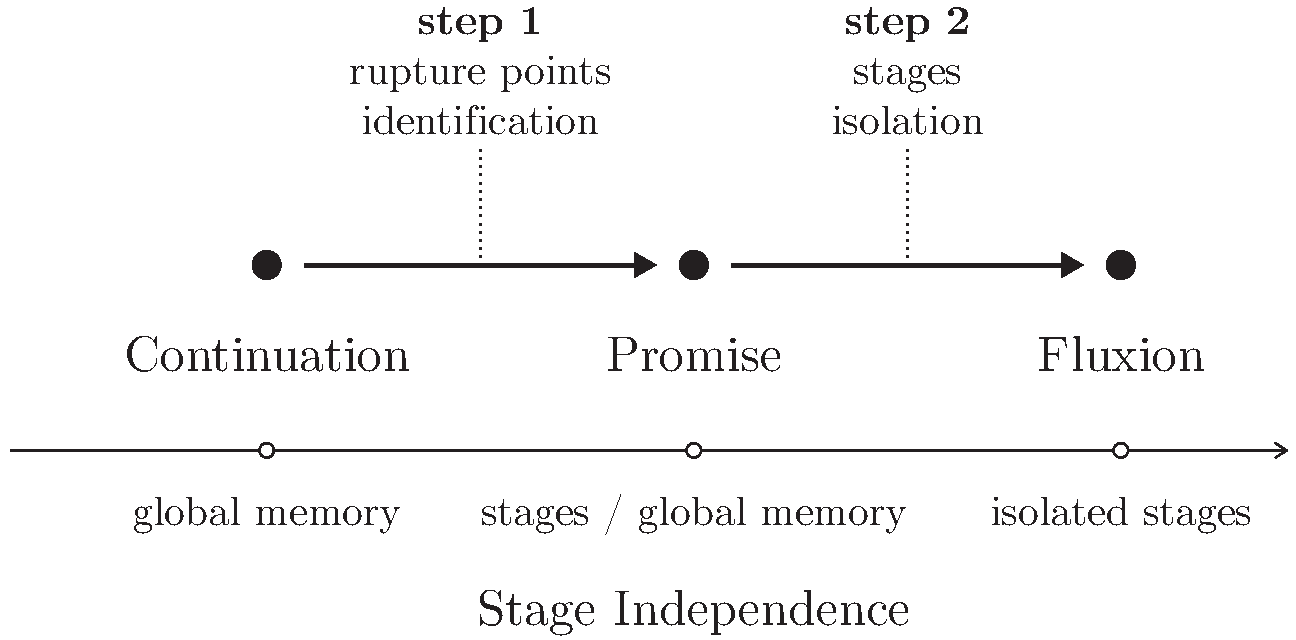
\includegraphics[width=0.9\textwidth]{../resources/roadmap.pdf}
\end{center}
\caption{Roadmap}
\label{fig:roadmap}
\end{figure}

\subsection{Rupture Point}

The pipeline architecture enforces the memory isolation between stages.
Each stage has its own thread of execution, and is independent from the others.
On the other hand, the execution flow of the event-loop jumps from one concurrent task to the other.
%  because of the continuation passing style and the common memory store.
% The message passing linking the callbacks is transparently handled by the event-loop.
However, the executions of these tasks are as distinct as the execution of the different stages of a pipeline.
The call stacks of two concurrent tasks are distinct.
The asynchronous function call between the caller and its continuation represents the rupture between two call stacks.
It is a rupture point, and is equivalent to a data stream between two stages in the pipeline architecture.

Both the pipeline architecture and the event-loop present these rupture points.
The detection of rupture points allows to map a pipeline architecture onto the implementation following the event-loop model.
To allow the transformation from one to the other, this thesis studies the possibility to detect rupture points, and to distribute the global memory into the parts defined by these rupture points.

The detection of rupture points is addressed in chapter \ref{chapter5}.
It presents the extraction of a pipeline of concurent tasks from a Javascript application.
Such pipeline is similar to the one exposed by Promises.
% The chapter proposes a simpler alternative to the latter called Dues.
However, these concurent tasks still require a global memory.
They can't be executed in parallel.

\subsection{Invariance}

% This transformation is important on two points.
% The conservation of the invariance.
% The equivalence between the coordinations.

The global memory assures the total ordering of tasks, and requires sequentiality, while message passing assures causal ordering of tasks and allows parallelism.
The causal ordering of tasks, by opposition to total ordering, is sufficient to assure the correctness of the execution.
Therefore, to assure the correctness of the execution, the ordering allowd by the global memory is partially equivalent to message passing ordering.
And it is possible to transform the global memory coordination into message passing.
% Given that the tasks are independent and communicate by messages.

% This result was used by Lamport to prove the correctness of distributed systems.
Yet, to preserve the correctness as expressed by the developer, it is important to preserve the invariance.
The global memory needs not to be distributed into each of the stages of the pipeline, so that each stage have an exclusive access to its memory.

To assure the missing coordinations assured by the shared memory between the stages, the transformation should provide equivalent coordination with message passing.
The isolation and replacement of the global memory is addressed in chapter \ref{chapter6}, with the introduction of isolated containers called Fluxions.




% The invariance holds for the whole memory during the execution of each callback.
% As I explained in the previous section, this invariance is required to allow the concurrent execution of the different tasks.
% On the other hand, the invariance is explicit in the pipeline architecture, as all the stages have isolated memories.
% The coordination between these isolated process is made explicit by the developer through message passing.

% I argue that the state coordination between the callbacks requireing a global memory could be replaced by the message passing coordination used manually in the pipeline architecture.
% I argue that not all applications need concurrent access on the state, and therefore, need a shared memory.
% % Specifically, I argue that each state region remains roughly local to a stage during its modification.
% \nt{TODO review that, I don't know how to formulate these paragraphs. Identify the state and the data in the global memory.}

% \subsubsection{Transformation}

% This equivalence should allow the transformation of an event loop into several parallel processes communicating by messages.
% In this thesis, I study the static transformation of a program, but the equivalence should also hold for a dynamic transformation.
% I present the analyzis tools I developed to identify the state and the data from the global memory.
# Explanation of the concept

## Turn-based programming.







(see presentation on Dues)
-> single-thread, no wait, no block and so on
Shared heap -> no mutex, no synchronization, so it is good scalability


Turn-based programming is an event-loop.
It is the execution of queued events one after the other.
An event is the association of a callback and a message.
The callback is a small Javascript Program, designed to process the message.
During its turn, the callback executes, and can queue events : that is register callback to be executed during a next turn.
TODO what I mean exactly by queue events ? -> the distinction between the asynchronous operation, and the resulting event.

## Pipeline

So a callback sends messages to other callbacks.
-> It is exactly like a pipeline.
However, all the callbacks share the same heap.
So it is not possible to distribute the different callbacks without synchronization of this heap, or splitting the heap for each callback.
TODO state VERY clearly this problem, it is at the core of my thesis.

So, how to split the heap so that each callback has its own exclusive heap ?

## Propagation of variables.

Javascript is lexically scoped, therefore we can identify the scope of variable statically.
(At the exception of eval and with : with is forbidden from strict mode, so that is not a bigdeal, howether, eval is sometimes used in smart ways, but most of the time it is monomorphic (I don't exactly know what that means, I heard from Floreat, it must be something related to PL community)).

### Scope identification

The compiler identifies the variables shared by multiple callbacks from their scope.
TODO explain this in depth.
Function scope, closures, and so on ...

### Scope leaking

Javascript uses a pass-by-sharing paradigm.
That means that sometimes the argument of a call are passed by value, sometimes by reference (atomic data type (number, string, bool) -> by value, complex data type (objects) -> by reference).
That means that the modification of a local variable can affect variable in seemingly unrelated scopes.
It seems that the points-to analysis is what is used to find stuffs like that (side-effects ?).

### Propagation of execution and variables

The execution progress downstream, following the message stream.
TODO state very clearly this proposition, it is the second core of my thesis (and I love the idea, it relates directly to reality, graivity, and the fabric of the universe <3).

Because the propagation of the modification is not instantaneous, going back upstream is like going backward in time : it is impossible.
Therefore, a variable cannot be read upstream a write.
And it cannot be write downstream either.

In other words, only one callback can write on a variable -> seems obvious from previous sections.


In promises, because the heap is not shared, things are less restrictive.
Multiple stages can read and write the same variable, because the propagation of modification is instantaneous, due to the shared heap.
\section{Overall Evaluation} \label{chapter6:evaluation}

The equivalence presented in chapter \ref{chapter4} is implemented in a the fluxional compiler, presented in section \ref{chapter5:flx}.
This implementation is evaluated against the criteria presented in chapter \ref{chapter3}, Productivity, Efficiency and Adoption.

\subsection{Trading Productivity for Efficiency}

% \subsubsection{Productivity}

The equivalence intends to disrupt as less as possible the way developer build web applications.
The goal is to avoid degrading the productivity, hence the adoption, of the proposed platform.
% The source language, Javascript, is left intact, except for the forbidden statements \texttt{with} and \texttt{eval}.
% These statements are already forbidden by some good practice guides \cite{Crockford2008}.
Therefore, the productivity is intended to be the same as the original event-driven platform.

However, in the current state, the compiler implementation is unable to operate the transformation without an external help.
The static analysis is unable to correctly detect the aliasing of the memory in Javascript.
It avoids developers to use Higher-Order Programming, hence impacts composition.
This limitation avoids to improve the current trade-off of productivity for efficiency, as illustrated in table \ref{tab:proposition-productivity}.
Indeed, to gain efficiency, developers need to commit efforts to indicate the stages of the pipeline, and assure their dependency.

% \TablePropositionProductivity{tab:proposition-productivity}

The manual transformation process yields a distributed application, similarly as the other efficient platforms.
And the chapter \ref{chapter3} showed that such applications achieve very good performance efficiency.
But the productivity limitation remains.
It avoids the current implementation to propose a satisfying compromise between productivity and efficiency.
So, the current implementation actually trades productivity for efficiency, similarly to many platform in the state of the art. % , as illustrated in table \ref{tab:proposition-efficiency}.
The perspectives to overcome this limitation are addressed later in section \ref{chapter5:evaluation:perspective}.
% \TablePropositionEfficiency{tab:proposition-efficiency}


% It doesn't make any sense to evaluate an application, as the transformation would not reflect the compilation process, but the manual transformation process.

% If the runtime memory analysis is solid enough to detect correctly the aliasing of the memory, then it will be able to help the development team transitioning from productivity to efficiency, which is the response of this thesis to the problematic.

\subsection{Adoption}

As observed in the chapter \ref{chapter3}, trading productivity for efficiency drastically reduces adoption.
Because the current implementation presents the same limitation than the efficient platforms, its adoption is not expected to be different. %, as illustrated in table \ref{tab:proposition-adoption}.

Yet, both productivity and efficiency are required for the platform to be adopted by new developers as well as large businesses.
Only at this condition, will it reinforce the loop between community and industry.
So the current implementation is not expected to be widely adopted, as presented in the table \ref{tab:proposition-summary}.

\TablePropositionSummary{tab:proposition-summary}
% \TablePropositionAdoption{tab:proposition-adoption}

% It was briefly tested during the development of the grumpy application, presented in chapter \ref{chapter4}, section \ref{chapter4:execution-models:examples}.

The limitation of static analysis avoids the equivalence to be fully implemented to address the problematic.
Hence, this evaluation holds only on the implementation, and not on the equivalence.


When saying that \textit{it is a mistake to attempt high concurrency without help from the compiler}, R. von Behren \textit{et al.} \cite{Behren2003} implies that the language alone cannot achieve high concurrency.
It is necessary to rely on additional tools, such as a compiler to reach the best compromise between productivity and efficiency.
The evaluation of this thesis concludes that static analysis is unable to reach this compromise for the current multi-paradigm languages using higher-order programming.
% Before dropping all higher-order languages for the sake of efficiency,
Yet, there exist alternatives to static analysis to reach this compromise.
The next paragraph presents some interesting perspectives of this work to further address this problematic.

% In the contribution of this thesis, the two main difficulties, identifying stages and detecting memory dependencies, are due to the dynamic nature of Javascript.
% A perspective to overcome these limitation is to implement the transformation, not as a compiler, but as a runtime.
% Indeed, at runtime, all the dynamic behavior are resolved, and the analysis can be much more precise, and less speculative.

% \subsection{Fluxionnal Runtime} 

% \section{Perspectives}

% Javascript is a highly dynamic languages.